\chapter{Analýza a realizace serverové aplikace}

Serverová aplikace je první ze dvou částí informačního systému. Tvoří centrum logické složky určené ve specifikaci a poskytuje veřejné \gls{api} pro všechny klientské aplikace. Realizuje logickou část uživatelského systému, systému oznámení, správy a hodnocení projektů, tvorby týmů a dalších požadavků. 

Daná kapitola popisuje tvorbu serverové RESTful\footnote{\gls{rest}} aplikace. Postupně jsou analyzovány, navrhovány a popisovány implementace vybraných části služeb. Pro tyto účely jsou v některých aspektech parciálně testovány webové frameworky, databáze a možná implementační řešení s následným výběrem nejvhodnějšího řešení.


% --------------------------------------------------------------------------------------------------
% Architektura aplikace
% --------------------------------------------------------------------------------------------------

\section{Architektura aplikace}

Základní komponentou informačního systému je serverová aplikace poskytující API pro klientské programy. Obsahuje větší část logického celku. Z hlediska funkcionality lze aplikaci rozdělit do následujících vrstev:

\begin{dl}
   \item [Datová vrstva] Datovou vrstvu definují datová úložiště a knihovny zprostředkovávající komunikaci mezi aplikací a úložišti.
   
   \item [Aplikační vrstva] Aplikační vrstva představuje logickou část aplikace. Je realizována zejména s pomocí middlewarů a pomocných utilit.
   
   \item [Prezentační vrstva] Prezentační vrstva v rámci dané aplikace není grafického typu. Představuje ji poměrně krátký zdrojový kód, jenž na základě obdržených dat generuje odpověď ve formátu \gls{json}, která je následně odeslána webovým frameworkem.
   
\end{dl}


Detailnějšímu návrhu architektury jsou věnovány následující podkapitoly, ve nichž je popsaný výběr nástrojů a způsob realizace některých funkcionalit.



% Výběr web frameworku
% --------------------------------------------------------------------------------------------------

\subsection{Webový aplikační framework}

Framework pro tvorbu \gls{api} je centrálním systémem serverové aplikace. Jeho volba do~jisté míry řídí celou architekturu, proto bylo rozhodnuto částečně zanalyzovat některé z nich pro výběr optimální varianty. Důležitá kritéria pro výběr byly:

\begin{ulnar}
   \item popularita na GitHub (existence komunity),
   \item minimalistické rozhraní (ne full-stack) frameworky,
   \item udržovaná a přehledná dokumentace,
   \item možnosti rozšíření frameworku dodatečnými utilitami.
\end{ulnar}


Na základě těchto faktorů byly vybrány pouze 4 frameworky, jež se techniky nejvíc hodí k implementaci serveru \gls{is}:

\begin{ulnar}
   \item express,
   \item koa,
   \item restify,
   \item fastify.
\end{ulnar}

Následný výběr byl řízen povrchovým testem rychlosti. S využitím každého frameworku byla napsána základní logická struktura~\ref{listing:speed-test-wf}, která se omezovala na jeden požadavek typu \texttt{GET} s jedním segmentem cesty a jedním parametrem. Výsledkem požadavku je vypsání odeslaného parametru s předpřipraveným textem.

\begin{fig:code}
	\begin{minted}{javascript}
const app = require('express')();

app.get('/path/:param', (req, res, next) => {
   res.send('Param: ' + req.params.param);
});

app.listen(3000);
   \end{minted}
   \caption{Příklad testované aplikace s využitím frameworku express}\label{listing:speed-test-wf}
\end{fig:code}

Alikace~\ref{listing:speed-test-wf} a obdobné realizace s pomocí jiných frameworků byly postupně spouštěny pro 10~000 požadavků s konkurencí 100 požadavků. Jako testovací zařízení byl použit Mac mini 2014:

\textbf{OS:} macOS Mojave 10.14.3\newline
\textbf{Procesor:} 2.5 GHz Intel Core i5\newline
\textbf{Operační paměť:} 8 GB 1600 MHz DDR3

Z výsledků testování~\ref{pic:chart-wf} vyplynulo, že framework express je v daných podmínkách nejlepší volbou, tudíž je vybrán pro implementaci \gls{is}. Daný nástroj bude použit i v realizaci klientské aplikace, kde je do jisté míry doporučován vybraným \gls{ssr} frameworkem, jenž s ním uvádí řadu příkladů v dokumentaci~\cite{nextExpress}.


\begin{fig:illustration}
   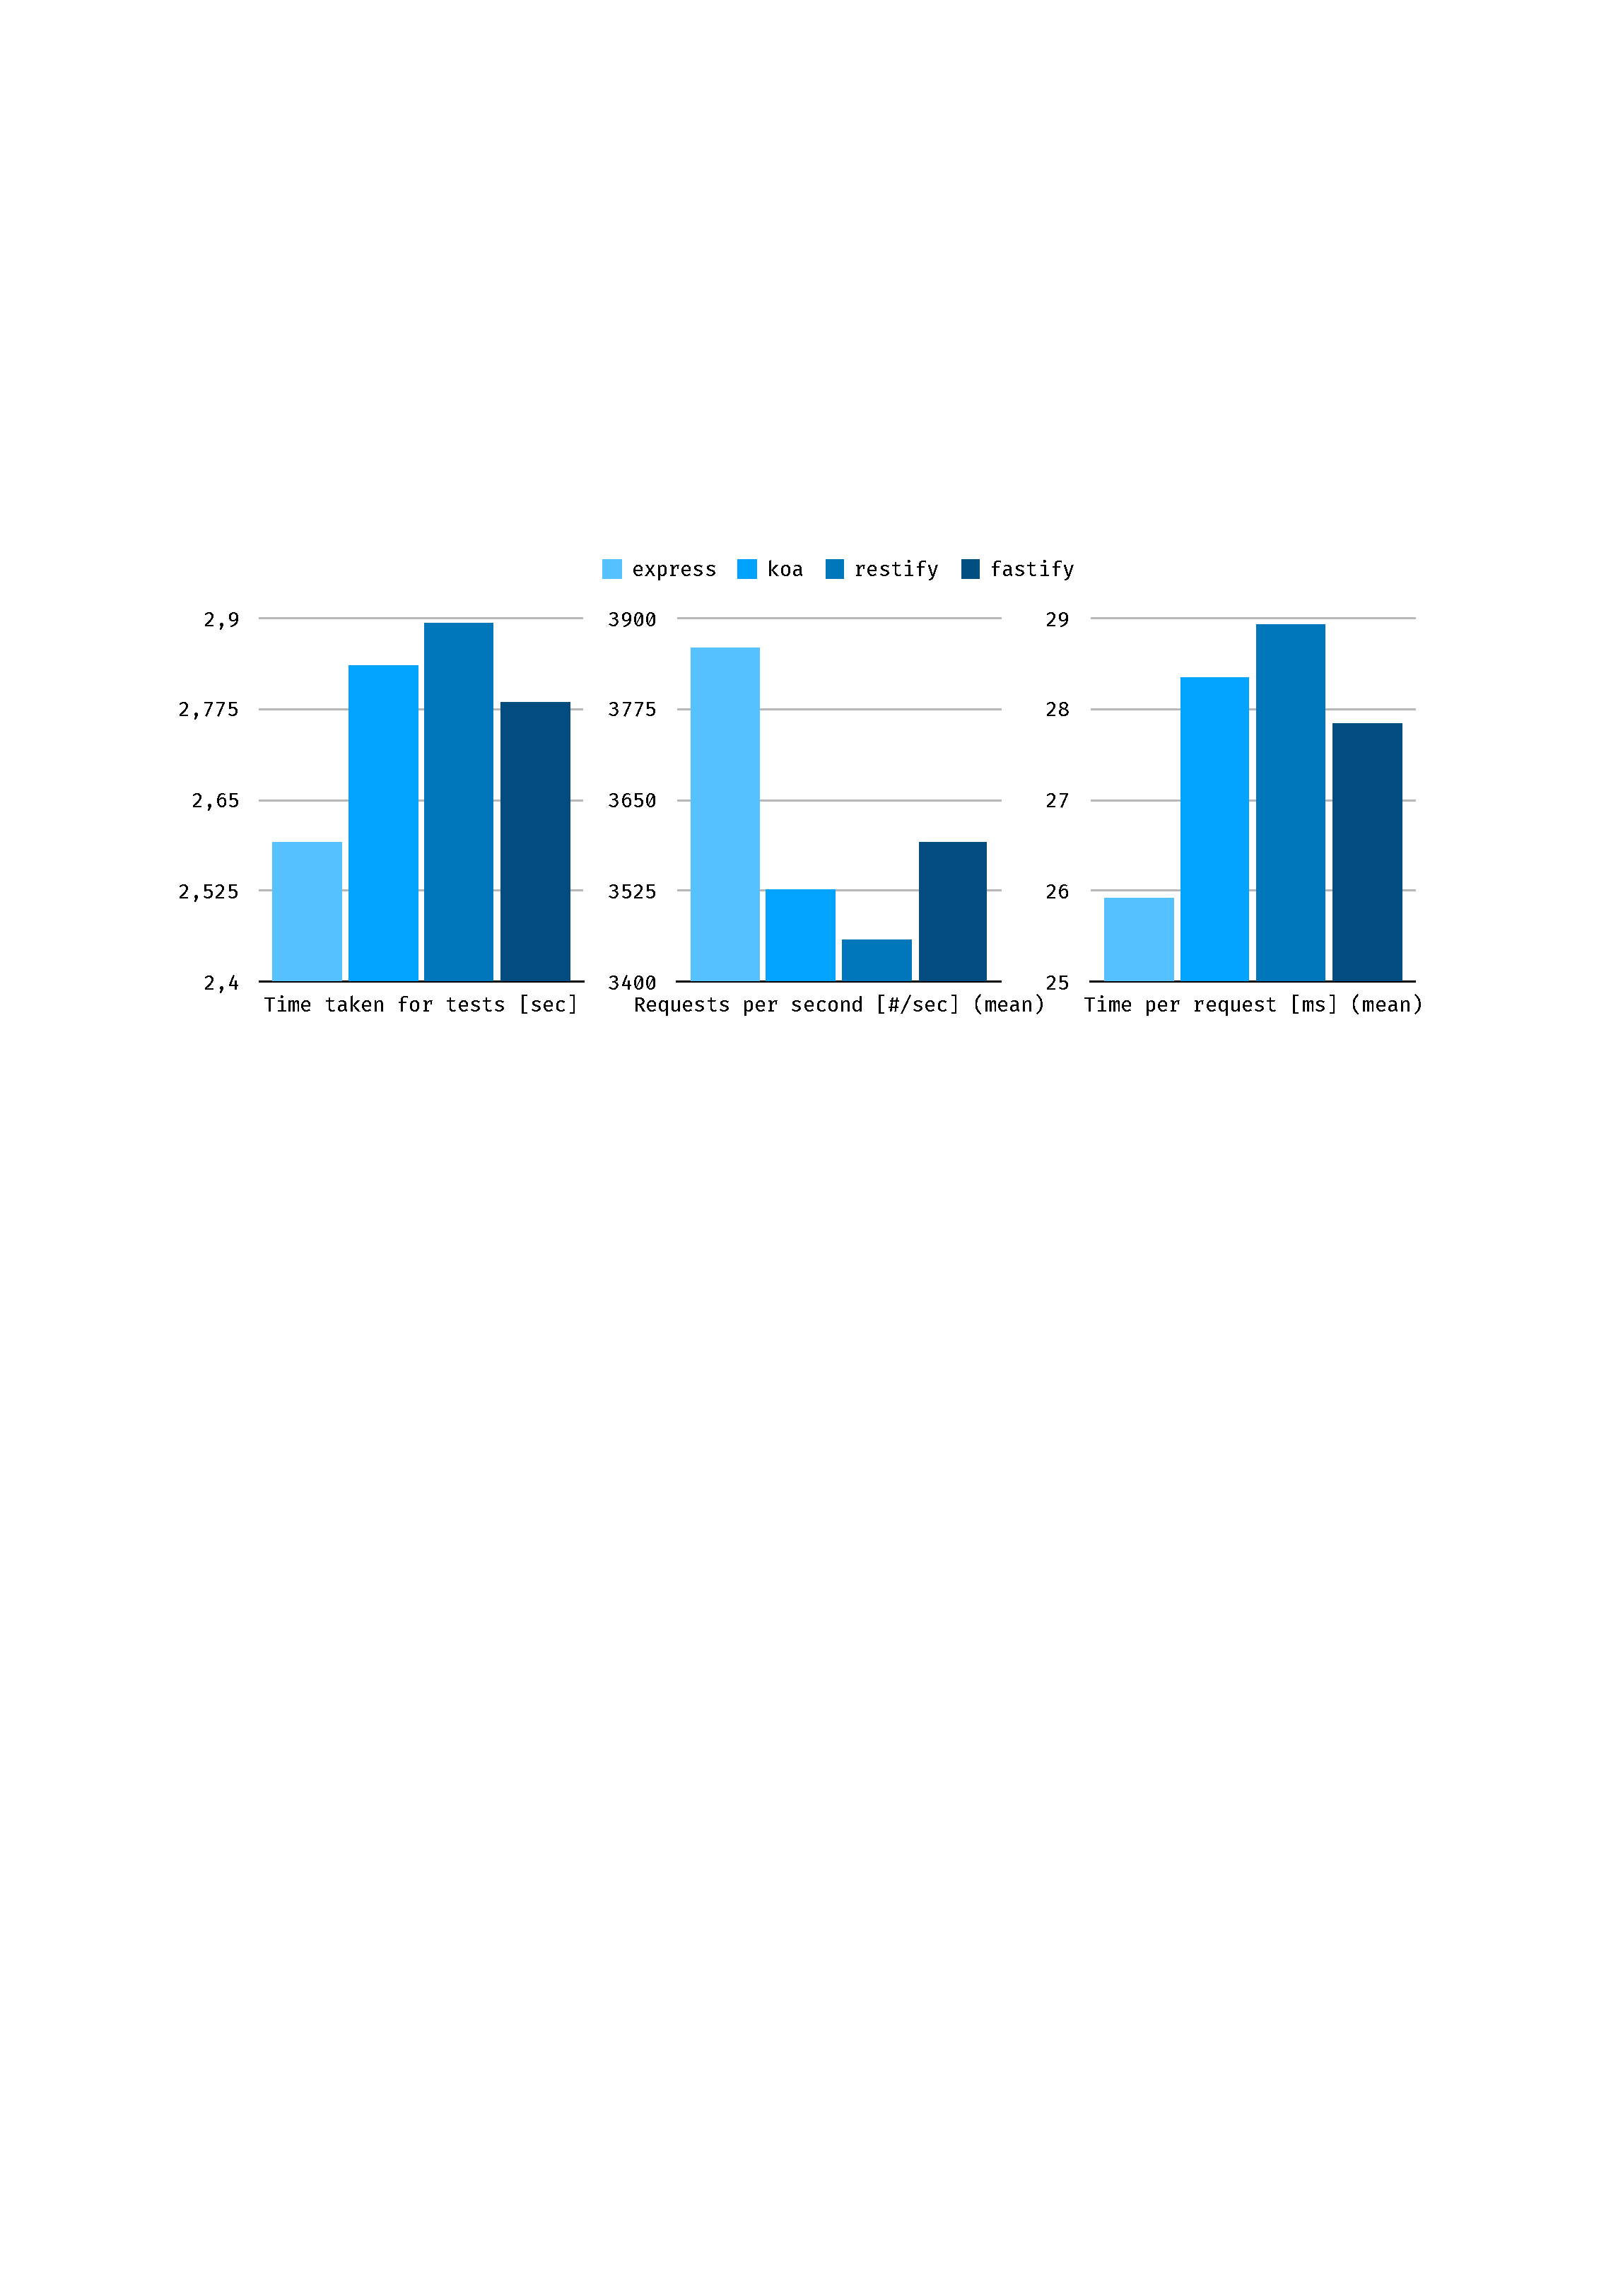
\includegraphics[width=1\textwidth]{images/chart-wf.pdf}
   \caption{Výsledky testování vybraných webových frameworků}\label{pic:chart-wf}
\end{fig:illustration}



% Datová úložiště
% --------------------------------------------------------------------------------------------------

\subsection{Datová úložiště}

Na základě specifikace lze definovat dva různé typy dat z hlediska využití. První skupina je tvořena například daty uživatelů, informacemi o projektu, snímkách obsahu apod. V této skupině je priorita kladena zachování závislostí neboli relací. Druhou skupinu tvoří text jednotlivých částí obsahu projektů. V tomto případě závislost je pouze jedna -- na projektu, mnohem důležitější je možnost ukládání velkých objemů dat s měnící se strukturou.

Pro první skupinu dat je víc vyhovující jedna z relačních databází, protože na rozdíl od \gls{nosql} databází samostatně spravuje cizí klíče a nabývá principů normalizace dat. Druhá skupina naopak vyžaduje jednu z \gls{nosql} databází pro správu dokumentů. Kromě volnější struktury modelů, které se v daném případě ideálně hodí pro ukládání částí obsahu, poskytuje možnost horizontálního škálování databáze~\cite{dbScaling}. Daná vlastnost bude vyžadována s rostoucími objemy uchovávaných dat, protože v porovnání s horizontálním škálováním, jenž je typické pro relační databáze, je méně náročná z hlediska potřebných zdrojů~\cite{dbScaling}.


Zástupci vhodných \gls{oss} relačních databází se staly MySQL a PostgreSQL. Vzhledem k mnoha existujícím článkům srovnání databází samostatná analýza nebyla potřeba. Výsledkem výzkumu jednoho z takových článků byl závěr, že oba zástupci \gls{dbms} jsou stejně stabilní, ale PostgreSQL poskytuje navíc podporu některých \gls{nosql} funkcionalit~\cite{mysqlPostgres}. Volbou \gls{nosql} databáze dle subjektivních zkušeností se stala MongoDB.


V průběhu implementace nastala potřeba definování dočasného úložiště pro výměnu autorizačních klíčů mezi serverem a klientem. Již zvolené databáze pro tento účel nebyly vhodnou volbou, protože by vznikla potřeba implementovat i démon pro automatické odstraňování předaných nebo nevalidních klíčů. Pro tento účel byla přidána další \gls{nosql} databáze Redis, která se zaměřuje na dočasné uchovávání dvojic klíč-hodnota.


Všechny databáze, až na Redis nejsou napřímo využívány \gls{is}. Prostředníkem komunikace aplikace s PostgreSQL je knihovna TypeORM. Jedná se o \gls{orm} knihovnu, jejíž úkolem je mapování databázových entit a jejich relací na objekty. Zjednodušuje obecnou komunikaci s databází a poskytuje rozhraní bez nutnosti psaní SQL příkazů. Mimo jiné zabezpečuje systém vůči útoku typu \uv{SQL injection}. Obdobná knihovna mongoose, která vzhledem k databázi je typu \gls{odm}, je využívaná pro komunikaci s MongoDB.


Stejně jako v případě samotné aplikace je nutné verzovat i strukturu vybraných databází, zejména PostgreSQL, protože obsahuje přesné struktury entit, na~rozdíl od~\mbox{MongoDB}, která je uchovává převážně ve volném \gls{json} objektu. Řešením jsou tzv. migrace -- soubory, jež uchovávají rozdíl stavů před a po jejich aplikování. Migrace v \gls{is} jsou plně řízeny knihovnou TypeORM. Všechny příkazy pro vytváření, spouštění a reset migrací jsou přidány do souboru \texttt{package.json}, jenž definuje základní \gls{cli} pro komunikaci s projektem.



% --------------------------------------------------------------------------------------------------
% Adresářová struktura
% --------------------------------------------------------------------------------------------------


\subsection{Adresářová struktura}

Adresářová struktura serverové aplikace je uvedená ve výpisu \ref{folders:server}. Představuje jednoduché rozdělení na funkční zdrojové kódy v adresáři \texttt{src} a testovací soubory v adresáři \texttt{test}, jenž kopírují strukturu \texttt{src} za účelem přehlednosti testovacích souborů. Adresáře \texttt{logs} a \texttt{tmp} uchovávají dočasné soubory, které nemají vliv na funkčnost aplikace.

\begin{fig:code}
   \begin{minted}{text}
.
├── logs            - logy aplikace
├── src
│   ├── api         - API routery
│   ├── config      - konfigurační soubory aplikace
│   ├── database    - modely, migrace, seed
│   ├── middlewares - middleware funkce
│   ├── routes      - statické routery
│   └── utils       - utility používané v aplikaci
├── test            - testovací soubory
├── tmp             - dočasné soubory
└── *.*             - inicializační a konfigurační soubory projektu
   \end{minted}
   \caption{Zkrácený výpis struktury složek klientské aplikace}\label{folders:server}
\end{fig:code}



% --------------------------------------------------------------------------------------------------
% Realizace funkcionalit
% --------------------------------------------------------------------------------------------------


% Realizace API
% --------------------------------------------------------------------------------------------------


\section{API}

Komunikace mezi serverem a klientem informačního systému probíhá prostřednictvím veřejně dostupného RESTful API. Důležitým faktorem je proto návrh intuitivně pochopitelné struktury \gls{uri}. Zásadním pravidlem se stalo třídění přistupovaných entit do skupin dle jejich nejběžnějšího výskytu. V případě různých operací nad stejnou entitou je využíváno různých \gls{http} metod:
\begin{dlnar}
   \item [GET] Získání dat.
   \item [POST] Vytvoření dat na základě určitých parametrů.
   \item [PATCH] Aktualizace dat.
   \item [DELETE] Trvalé nebo dočasné odstranění dat.
\end{dlnar}


Pro generování odpovědi ze strany serveru je využívána šablona~\ref{response-template}. Položka \texttt{typ} označuje stav odpovědi -- úspěšná nebo neúspěšná --, \texttt{msg} obsahuje krátkou zprávu o výsledku prováděné činnosti, objekt \texttt{dat} nese v sobě užitečné informace, kvůli kterým byla volaná \gls{api} metoda. Tento typ odpovědi není optimální z hlediska přenášení zbytečnych dat, byl ale zvolen kvůli zvýšení informativnosti odpovědi. Pro dokumentování \gls{api} je vybrána aplikace Postman, exportovaná dokumentace je uložena na přiložené médiu.


\begin{fig:code}
   \begin{minted}{javascript}   
{
   typ: "",
   msg: "",
   dat: {},
}
   \end{minted}
   \caption{JSON šablona pro odpověd serveru na uživatelský požadavek}\label{response-template}
\end{fig:code}



Vzhledem k veřejnému API je zřejmé, že k serveru budou přistupovat různé domény, případně stejná doména, jako má server, ale s odlišným portem. V běžném prostředí dochází k blokování sdílení informací mezi různými doménami kvůli bezpečnosti. Dané omezené je kladeno mechanismem \gls{cors}.~\cite{corsActions}

Pro povolení využití sdílení zdrojů je třeba na straně serveru nastavit speciální hlavičky, jež budou odesílány se všemi odpovědi na požadavky. Na serveru \gls{cors} řeší speciální middleware spouštěný před každým zpracováním požadavku od klienta. Příklad nastavení \gls{http} hlaviček je uveden v ukázce~\ref{listing:cors-access}.


\begin{fig:code}
	\begin{minted}{javascript}
res.header(
   'Access-Control-Allow-Origin', 
   '*');
res.header(
   'Access-Control-Allow-Methods', 
   'GET, POST, PATCH, PUT, DELETE, OPTIONS');
res.header(
   'Access-Control-Allow-Headers', 
   'Origin, Accept, Content-Type, Authorization');
   \end{minted}
   \caption{Nastavení HTTP Access-Control-Allow hlaviček}\label{listing:cors-access}
\end{fig:code}


Speciálním případem požadavku je \texttt{preflight}. Jedna se o HTTP požadavek typu \texttt{OPTIONS}, jenž se posílá samostatně na každé stránce před potřebným požadavkem~\cite{corsActions}. Zjišťuje povolené domény, metody a jiné hlavičky. \texttt{Preflight} požadavek musí být vždy úspěšný, proto spolu s \gls{cors} hlavičkami je v middlewaru odchytáván před jakýmkoliv dalším zpracováním, aby  bylo zajištěno, ze daný typ požadavku vždy proběhne a vrátí parametry serveru. Implementaci detekování a návrat hodnoty lze vidět na ukázce~\ref{cors-preflight}.


\begin{fig:code}
   \begin{minted}{javascript}   
if (req.method === 'OPTIONS')
   return res.status(200).end();
   \end{minted}
   \caption{Zpracování \texttt{preflight} požadavku}\label{cors-preflight}
\end{fig:code}




% Realizace uživatelského systému
% --------------------------------------------------------------------------------------------------

\section{Uživatelský systém}

Dle specifikace aplikace implementuje samostatný uživatelský systém s funkcionalitou přístupových práv, nemá však vlastní autorizační server. Místo toho využívá vnější servery třetích stran. Pro ukázkovou implementaci byl vybrán veřejný autorizační server GitHub OAuth 2.0, implementace ale počítá s připojením neomezeného množství obdobných služeb. Komunikace je zajištěna frameworkem PassportJS, jenž pro úplnou konfiguraci potřebuje pouze definování způsobu mapování dat uživatele z autorizačního serveru na entitu \gls{is}. 

Po úspěšném přihlášení či registraci uživatele přes vybraný autorizační server vzniká potřeba autorizované komunikace mezi klientskou aplikací a serverem, proto je nutné zvolit způsob identifikace uživatele v systému. Jedním ze způsobů identifikace je využívání unikátního klíče během každého požadavku na server. Knihovna JSON Web Token slouží ke generování a ověřování takových klíčů. \gls{jwt} funguje na principu digitálních podpisů, tím jsou řešeny situace s udržování a správou uživatelských klíčů na straně serveru. Pro úspěšnou autorizaci je nutné pouze ověření digitálního podpisu během každého uživatelského požadavku. Veškerá následující činnost uživatele je řízena jeho právy v rámci \gls{is}.

